\section{Lezione 26 - 21/11/2023}
\subsection{Grafi Pesati}
I \textbf{grafi pesati} come dice la parola si differenziano dai grafi normali per la presenza di pesi sugli archi, andremo ad indicarlo nel seguente modo:
$$ G=(V,E,w)$$
in cui $w$ è una "funzione" che associa ad ogni arco un numero reale (peso)
$$ w: E \rightarrow \mathbb{R}$$
Preso un generico percorso $\pi=v_1v_2v_3...v_k$ il peso di questo percorso sarà dato da:
$$ w(\pi)=\sum_{i=1}^{k-1} w(v_i,v_{i+1})$$
In questa tipologia di struttura è molto utile andare a calcolare il \textbf{percorso minimo}, cioè l'insieme di archi che collegano un vertice $u$ ad un vertice $v$ che sommati hanno il peso minore, possiamo indicarlo così:
$$ \delta(u,v)$$ 
il peso del percorso da u a v con peso minimo (possiamo chiamarlo anche lunghezza)

\paragraph{Esempio 1} Prendiamo come riferimento questo grafo pesato:
\begin{figure}[H]
	\centering
	\begin{subfigure}[b]{0.25\textwidth}
		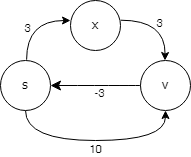
\includegraphics[width=\textwidth]{GrafoPesato01} 
		%\caption{Grafo non Connesso}
	\end{subfigure}
\end{figure} 
prendiamo un percorso $\pi=sxv$ il suo peso sarà $w(\pi)=3+3=6$ questo è il \textbf{percorso minimo} da $s$ a $v$, un altro esempio di percorso $\pi^{\prime}=sxvsxv$ avrà peso $w(\pi^{\prime}) = 9$

\paragraph{Esempio 2} Prendiamo invece questo grafo con pesi negativi
\begin{figure}[H]
	\centering
	\begin{subfigure}[b]{0.25\textwidth}
		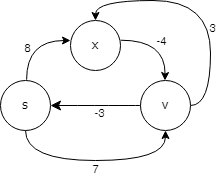
\includegraphics[width=\textwidth]{GrafoPesato02v} 
		%\caption{Grafo non Connesso}
	\end{subfigure}
\end{figure} 
In questo caso \textbf{non esiste un percorso minimo da $s$ a $v$} poiché:
$$ \pi=sxv \; w(\pi) = 4$$
$$ \pi=sxvxv \; w(\pi) = 3$$
$$ \pi=sxvxvxv \; w(\pi) = 2$$
possiamo notare come il peso va sempre a diminuire quindi non c'è un percorso minimo, dovuto dalla preso di un ciclo a peso negativo che ad ogni "iterazione" fa diminuire di unità il peso.\bigskip

\underline{Il problema del percorso minimo non è presente nei grafi privi di cicli a peso negativo}

\subsection{Algoritmi visita Grafi Pesati}
Dato un grafo pesato tramite un Algoritmo di visita BFS possiamo andare a calcolare la stima del peso di un percorso $\pi$, ne possiamo distinguere due:
\paragraph{Algoritmo di Dijkstra} è usato solo per grafi con pesi non negativi.
\paragraph{Algoritmo Bellman-Ford} per grafi pesati arbitrari.
Entrambi sono basati sul concetto di "rilassamento" degli archi.

\subsection{Rilassamento}
Il rilassamento è una tecnica che consente di stimare il percorso con peso minore.\smallskip

Consideriamo la funzione:
$$ d: V \rightarrow \mathbb{R} $$
che ad ogni vertice viene associato un reale che corrisponde a una stima del peso.
\begin{lstlisting}[language=Java]
relax(u,v,w):
    if d[v] > d[u] + w(u,v) then //d: distanza, w: peso
        d[v]=d[u]+w(u,v)
        pred[v]=u
\end{lstlisting}
Se la nuova stima è migliore aggiorno, ovviamente esistono casi in cui la stima è migliore anche se bisogna percorrere più archi.

\subsection{Propietà Percorsi Minini su Grafi Pesati}
\subsubsection{Lemma 1}
Dato $G=(V,E,w)$ e $\pi=v_1v_2...v_{k-1}v_k$ percorso minimo da $v_1$ a $v_k$ allora:
$$ \forall 1 \le i \le j \le k, \pi_{ij}=v_iv_{i+1}...v_j$$
$$ \pi_{ij} \text{ è un percorso minimale da } v_i \text{ a } v_j$$
Ogni percorso minimo tra due qualsiasi vertici  è formato da percorsi minimi ad altri vertici. Non è possibile che un percorso minimo tra due vertici contenga all'interno una sequenza che non è percorso minimo.

\paragraph{Dimostazione}
\blindtext

\subsubsection{Corollario 1}
Dato $G=(V,E,w)$ e $\pi=v_1v_2...v_{k-1}v_k$ percorso minimo da $v_1$ a $v_k$ allora:
$$ \delta(v_1,v_k) = \delta(v_1,v_{k-1})+w(v_{k-1},v_k) $$
La distanza tra due vertici è il peso del percorso più corto tra i due.

\paragraph{Dimostazione}
$$ \pi = \underbrace{v_1v_2...v_{k-1}}_{\pi_{1 k-1}}v_k$$
$$ w(\pi) = \delta(v,v_k)$$
\begin{center}
    Per il Lemma 1: $ w(\pi_{1 k-1}) = \delta(v_1,v_{k-1})$    
\end{center}

\subsubsection{Lemma 2 (Disuglianza Triangolare)}
Dato $G=(V,E,w)$ e $s \in V$ per ogni arco $(u,v) \in E$ abbiamo che:
$$ \delta(s,v) \le \delta(s,u)+w(u,v) $$
Il percorso minimo che va da $s$ a $v$ non può essere più lungo del percorso minimo da $s$ ad $u$ con aggiunto l'arco $u,v$.
\paragraph{Dimostazione} Banale.

\subsection{Proprietà di Relax}
\subsubsection{Lemma 3}
Dato  $G=(V,E,w)$ e $(u,v) \in E$, immediatamente dopo l'esecuzione di relax(u,v,w) avremo che:
$$ d[v] \le d[u]+w(u,v)$$
\paragraph{Dimostazione} Banale.

\subsubsection{Lemma 4}
Dato  $G=(V,E,w)$ e posti $d[v]=\infty$ e $\forall v \in V \backslash\{s\}$ e $d[s]=0$ lungo una qualsiasi sequenza di operazioni di rilassamento avremo che:
$$ d[v] \ge \delta(s,v) \forall v \in V$$
In pratica non possiamo mai sottostimare.

\paragraph{Dimostazione} Induzione sul numero delle operazioni di rilassamento \smallskip

\textbf{Caso base i=0} banale \medskip

\textbf{Passo induttivo i > 0} Ipotesi: prima i-esima operazione $\forall v \in V d[v] \ge \delta(s,v)$. \smallskip

Eseguiamo relax(x,y,w), poiché modifica solo $d[y]$ sicuramente:
$$ \forall v \in V \backslash\{y\} \; d[v] \ge \delta(s,v) $$
Abbiamo due possibilità casi prima di relax:
\begin{itemize}
    \item 1) $d[y] \le d[x]+w(x,y)$ allora $d[y] \ge \delta(s,y)$ (per ipotesi)
    \item 2) $d[y] > d[x]+w(x,y)$ allora $d[y]=d[x]+w(x,y)$
\end{itemize}
DA RIVEDERE
$$ d[y] \ge \delta(s,x)$$
$$ \delta(s,x) \le \delta(s,x)+w(x,y)$$

\subsubsection{Corollario 2}
Se $v$ non è raggiungibile da $s$ (con inizializzazione delle stime ad $\infty$ e $0$), in ogni momento lungo una sequenza arbitraria di rilassamenti vale:
$$ d[v]=\delta(s,v)$$
\paragraph{Dimostazione} Se $v$ non è raggiungibile da $s$ allora $\delta(s,v)=\infty$ \smallskip

Per il lemma 4 $d[v] \ge \delta(s,v) \forall v \in V$ quindi avremo:
$$ d[v]=\delta(s,v)=\infty$$

\subsubsection{Lemma 5}
Dato $G=(V,E,w)$ e $\pi=v_1v_2...v_{k-1}v_k$ percorso minimo da $v_1$ a $v_k$, inizializzando $d[v]=\infty$ e $d[v_1]=0$, presa un arbitraria sequenza di rilassamenti che contiene \textbf{relax($v_{k-1}, v_k, k$)}, se prima di relax $d[v_{k-1}]=\delta(v_1,v_{k-1})$ allora dopo relax $d[v_k]=\delta(v_1,v_k)$
\paragraph{Dimostazione} \blindtext